\subsection{Layers}
\label{sec:layers}

\subsubsection{Layer size distribution}

\begin{figure}[!t]
	\centering
	\subfigure[CDF of layers by layer size]{\label{fig_layer_size_cdf}
		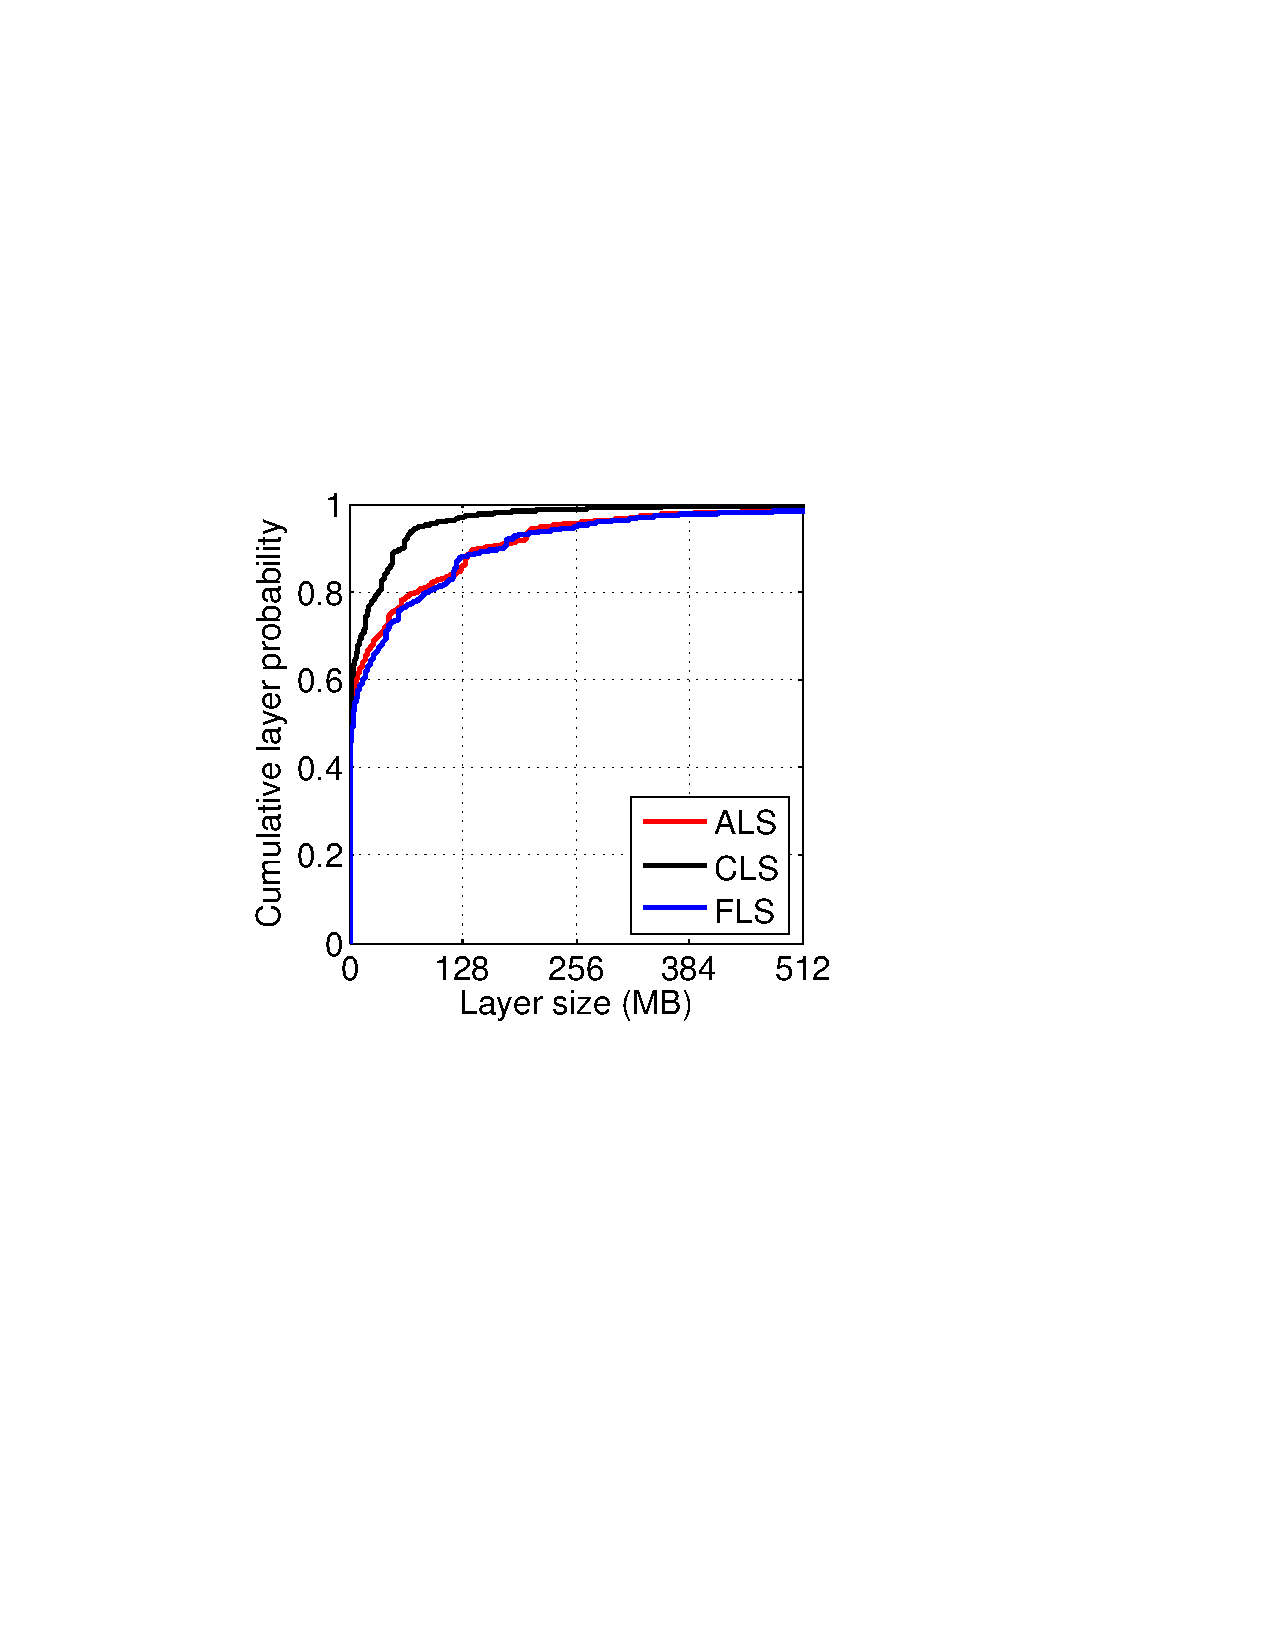
\includegraphics[width=0.23\textwidth]{graphs/layer_size_mb.pdf}
	}
	\subfigure[Histogram of layers by layer size]{\label{fig_hist_layer_size}
		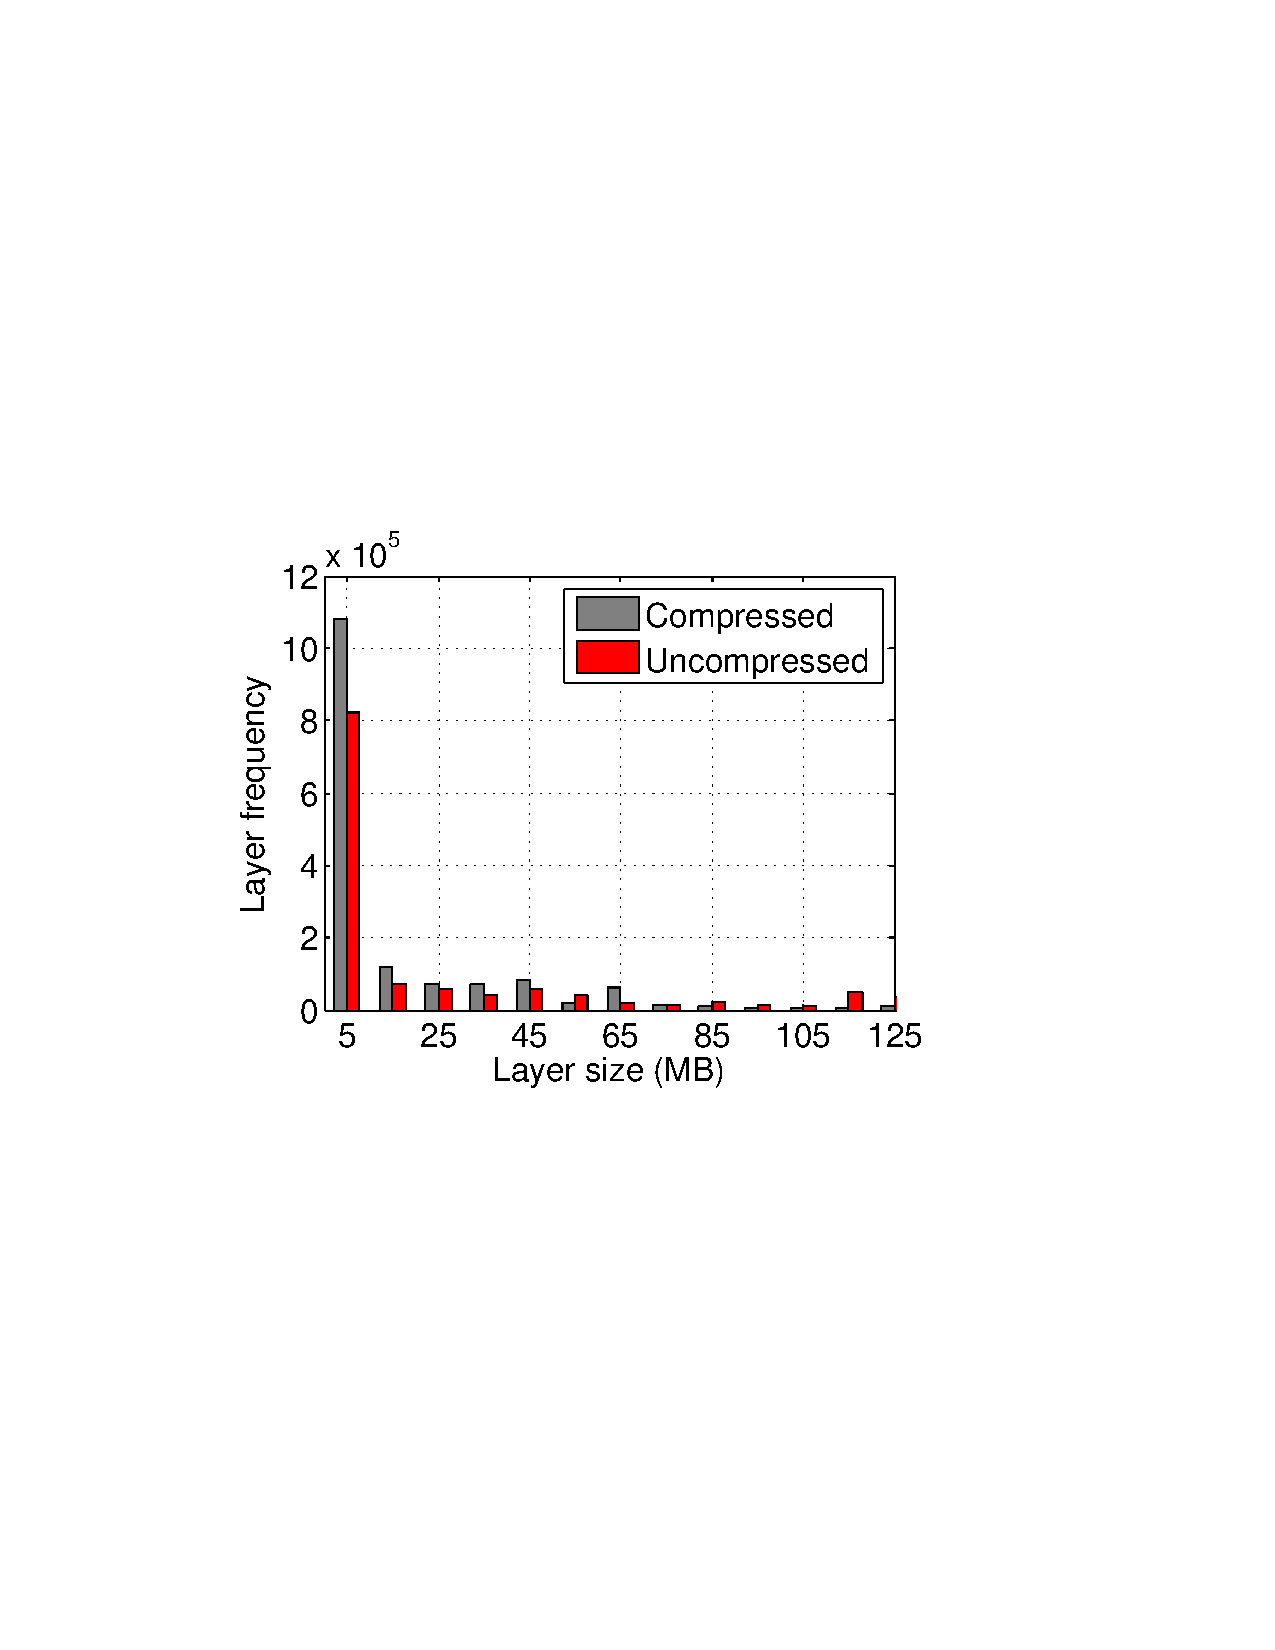
\includegraphics[width=0.223\textwidth]{graphs/hist_layer_size.pdf}
	}
	\caption{Layer size distribution}
	\label{fig-layer-size}
\end{figure}

Like image size, we also measured three kinds of layer size: archival size, compression size, and the sum of containing file size. Compression size is the original layer size after downloaded; The archival size is the decompressed layer size without extracting and unpacking; The sum of containing file size is the sum of its containing file size after decompression with extracting and unpacking.

Figure~\ref{fig_layer_size_cdf} shows the cumulative layer probability by layer size for three kinds of layer size.
As shown in figure~\ref{fig_layer_size_cdf}, the red curve and blue curve are almost overlapped, which means that the distribution of archival size and the distribution of sum of file size are similar. 90\% of layers have a less than 177 MB uncompression size (i.e., archival size or the sum of containing file size), while 90\% of layers have a less than 63 MB compression size. Half of layers are less than ~4 MB (i.e., uncompression size or compression size). The largest uncompression image size is ~29 GB (23 GB for the sum of file size) while the largest compression size is only 19 GB.
Figure~\ref{fig_hist_layer_size} shows the histogram of layer by layer size. About 1,080,000 of the layers' compression size is less than 5 MB while 985,000 layers' archival size less than 5 MB, 820,000 layers' sum of file size is less than 5 MB. 
Figure~\ref{fig-layer-size} shows that the majority of the layers in Docker hub have a smaller size. 90\% of layer can be compressed with less than 63 MB and 77\% of images are less than 63 MB even without compression. 

\subsubsection{Layer compression ratio distribution}

\begin{figure}[!t]
	\centering
	\subfigure[CDF of layers by layer size]{\label{fig_cdf_compression_ratio}
		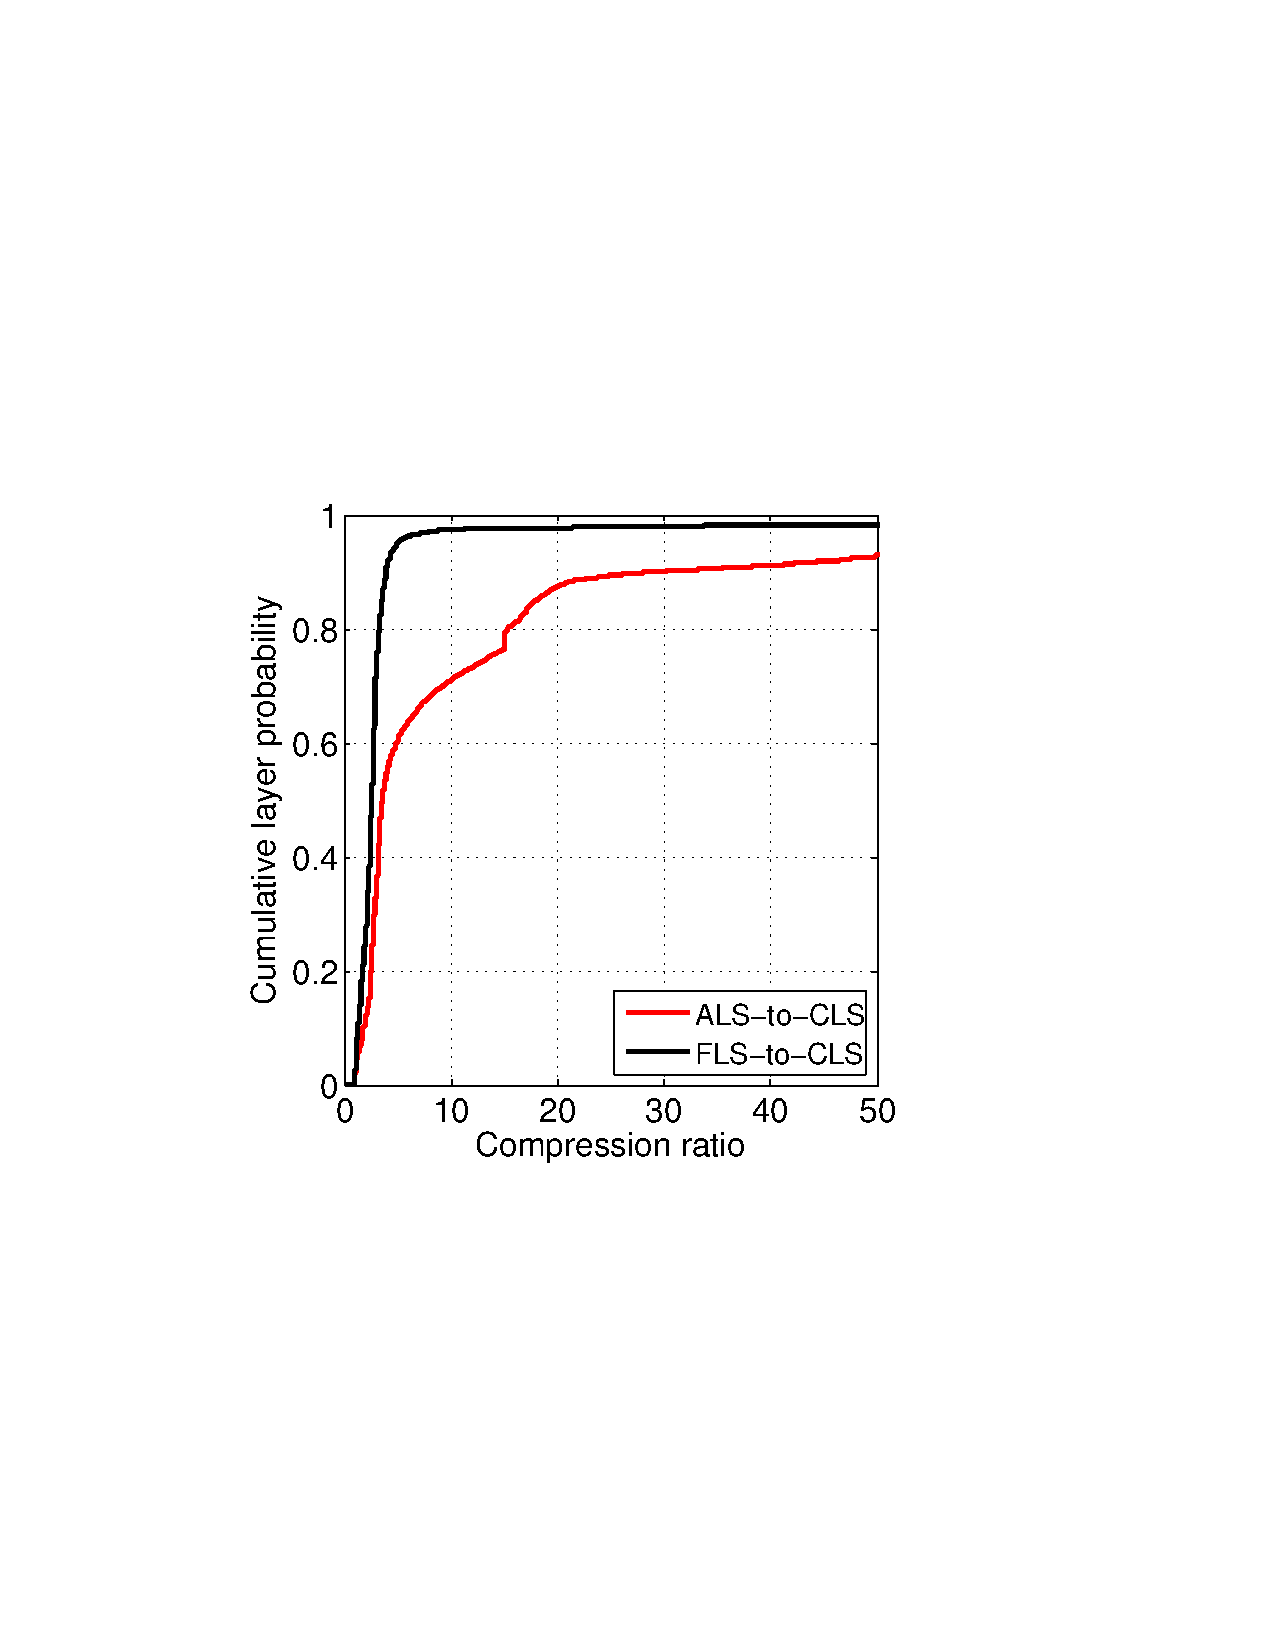
\includegraphics[width=0.23\textwidth]{graphs/cdf_compression_ratio.pdf}
	}
	\subfigure[Histogram of layers by layer size]{\label{fig_his_compression_ratio}
		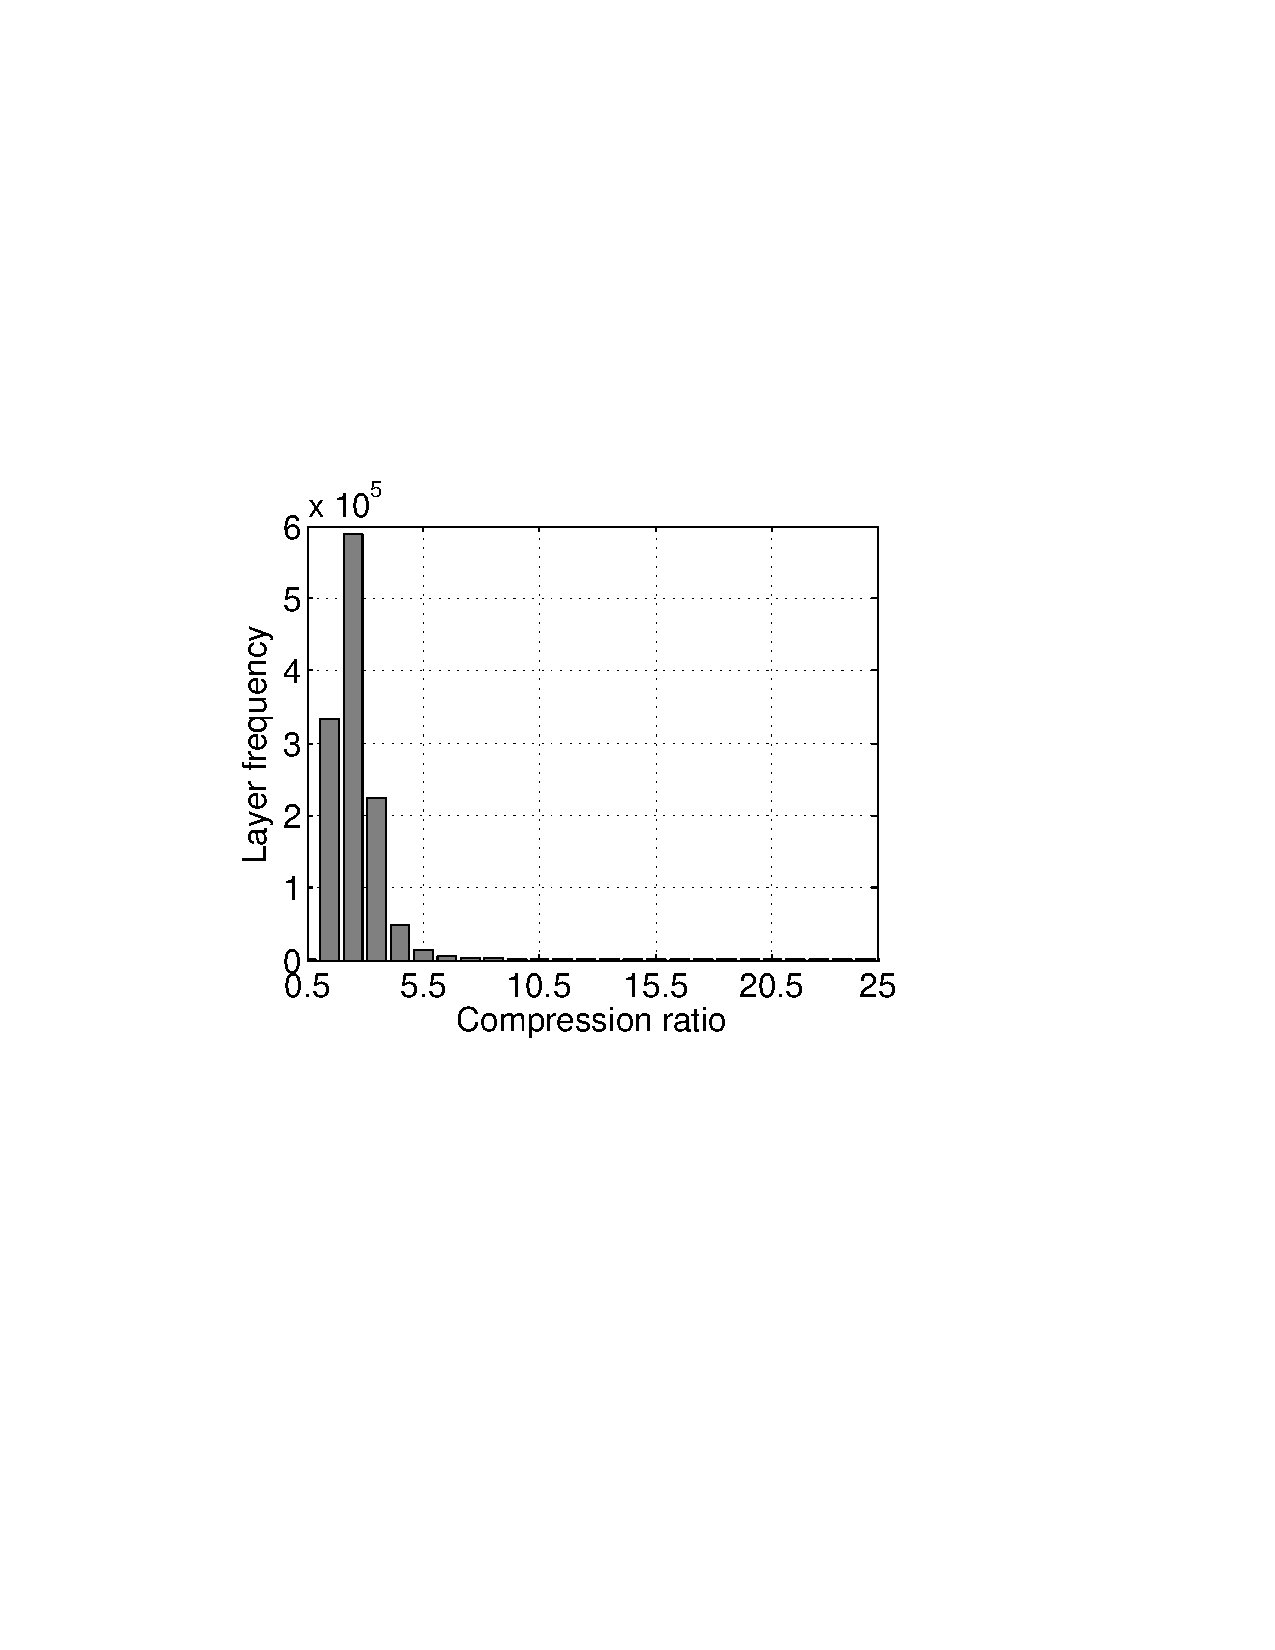
\includegraphics[width=0.223\textwidth]{graphs/his_compression_ratio.pdf}
	}
	\caption{Layer compression ratio distribution}
	\label{fig-compression-ratio}
\end{figure}

Since three kinds of layer size are measured: archival size, compression size, and the sum of containing file size. Thus, we calculated two kinds of compression ratio: the ratio of archival size to compression size and the ratio of Sum of file size to compression size. 

Figure~\ref{fig_cdf_compression_ratio} shows the cumulative layer probability by compression ratio. Overall, we can see that the ratio of archival size to compression size is greater than the ratio of the sum of file size to the compression size. 90\% of images have a archival-to-compression ratio less than ~4 while 90\% of images have a sum of file-to-compression ratio less than 30. Half of the images have a compression ratio (both archival-to-compression and sum of files-to-compression) around 3. The maximum compression ratio are 512,930 and 1026 for the ratio of sum to file size to compression size and the ratio of archival to compression size respectively.
Figure~\ref{fig_his_compression_ratio} shows a histogram of layer by compression ratio. 587,000 images have a ratio of sum of file size to compression size of 3 and 331,000 images have a ratio of archival size to compression size of 3, which are two peaks shown in the graph.

Figure~\ref{fig-compression-ratio} suggests that layers have a great potential for compression to save space.

\subsubsection{Layer depth distribution}

After extracting and unpacking gzip compressed layer archival files, we calculated the layer directory depth (i.e., the maximum directory depth). 
Figure~\ref{fig_layer_depth} shows the cumulative layer probability by layer directory depth. Around 90\% of layers' directory depth is less than 10. 50\% of layers' directory depth is less than 4. 

Figure~\ref{fig_hist_layer_depth} shows the histogram of layers by layer directory depth. About 313,000 layers' layer directory depth is 3, which is the peak value in the figure. The maximum repeat count is 444 while the median is 4. The average is ~5.

\begin{figure}[!t]
	\centering
	\subfigure[CDF of layers by layer directory depth]{\label{fig_layer_depth}
		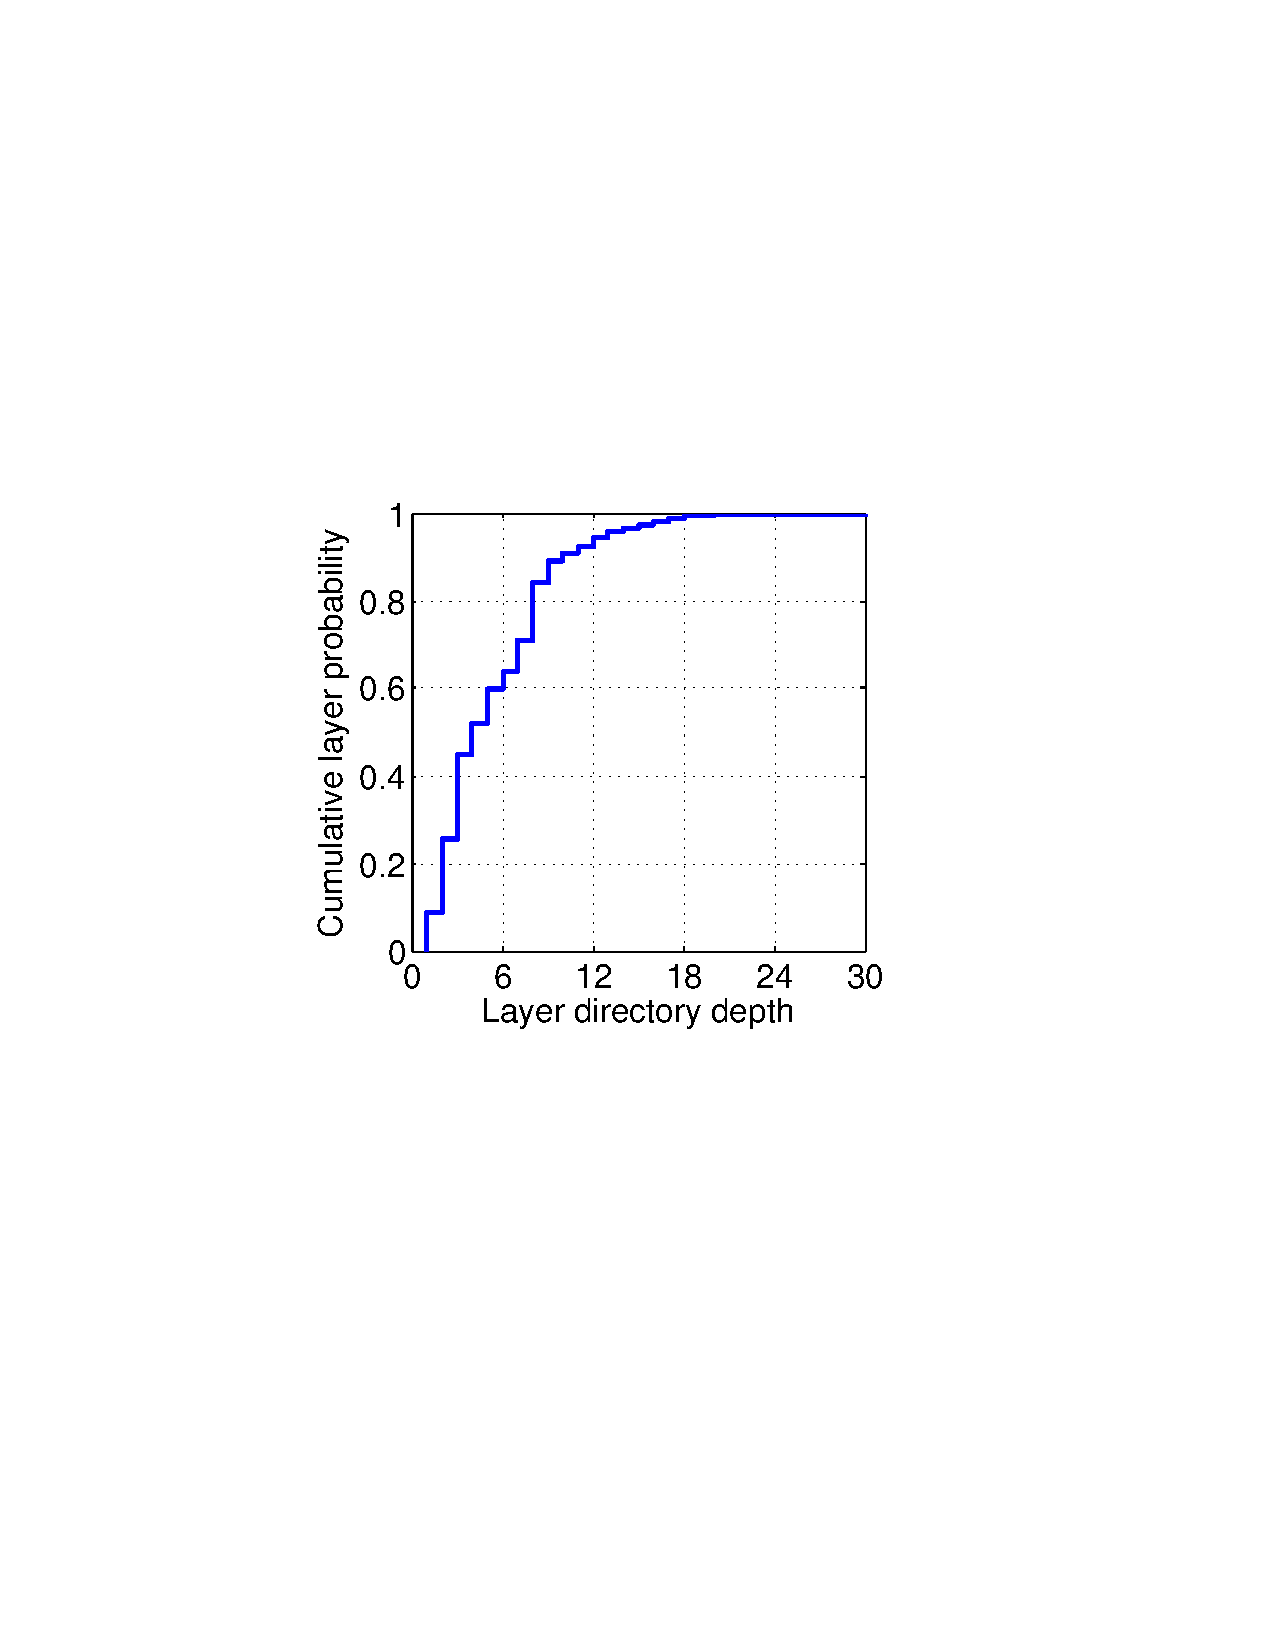
\includegraphics[width=0.23\textwidth]{graphs/layer_depth.pdf}
	}
	\subfigure[Histogram of layers by layer directory depth]{\label{fig_hist_layer_depth}
		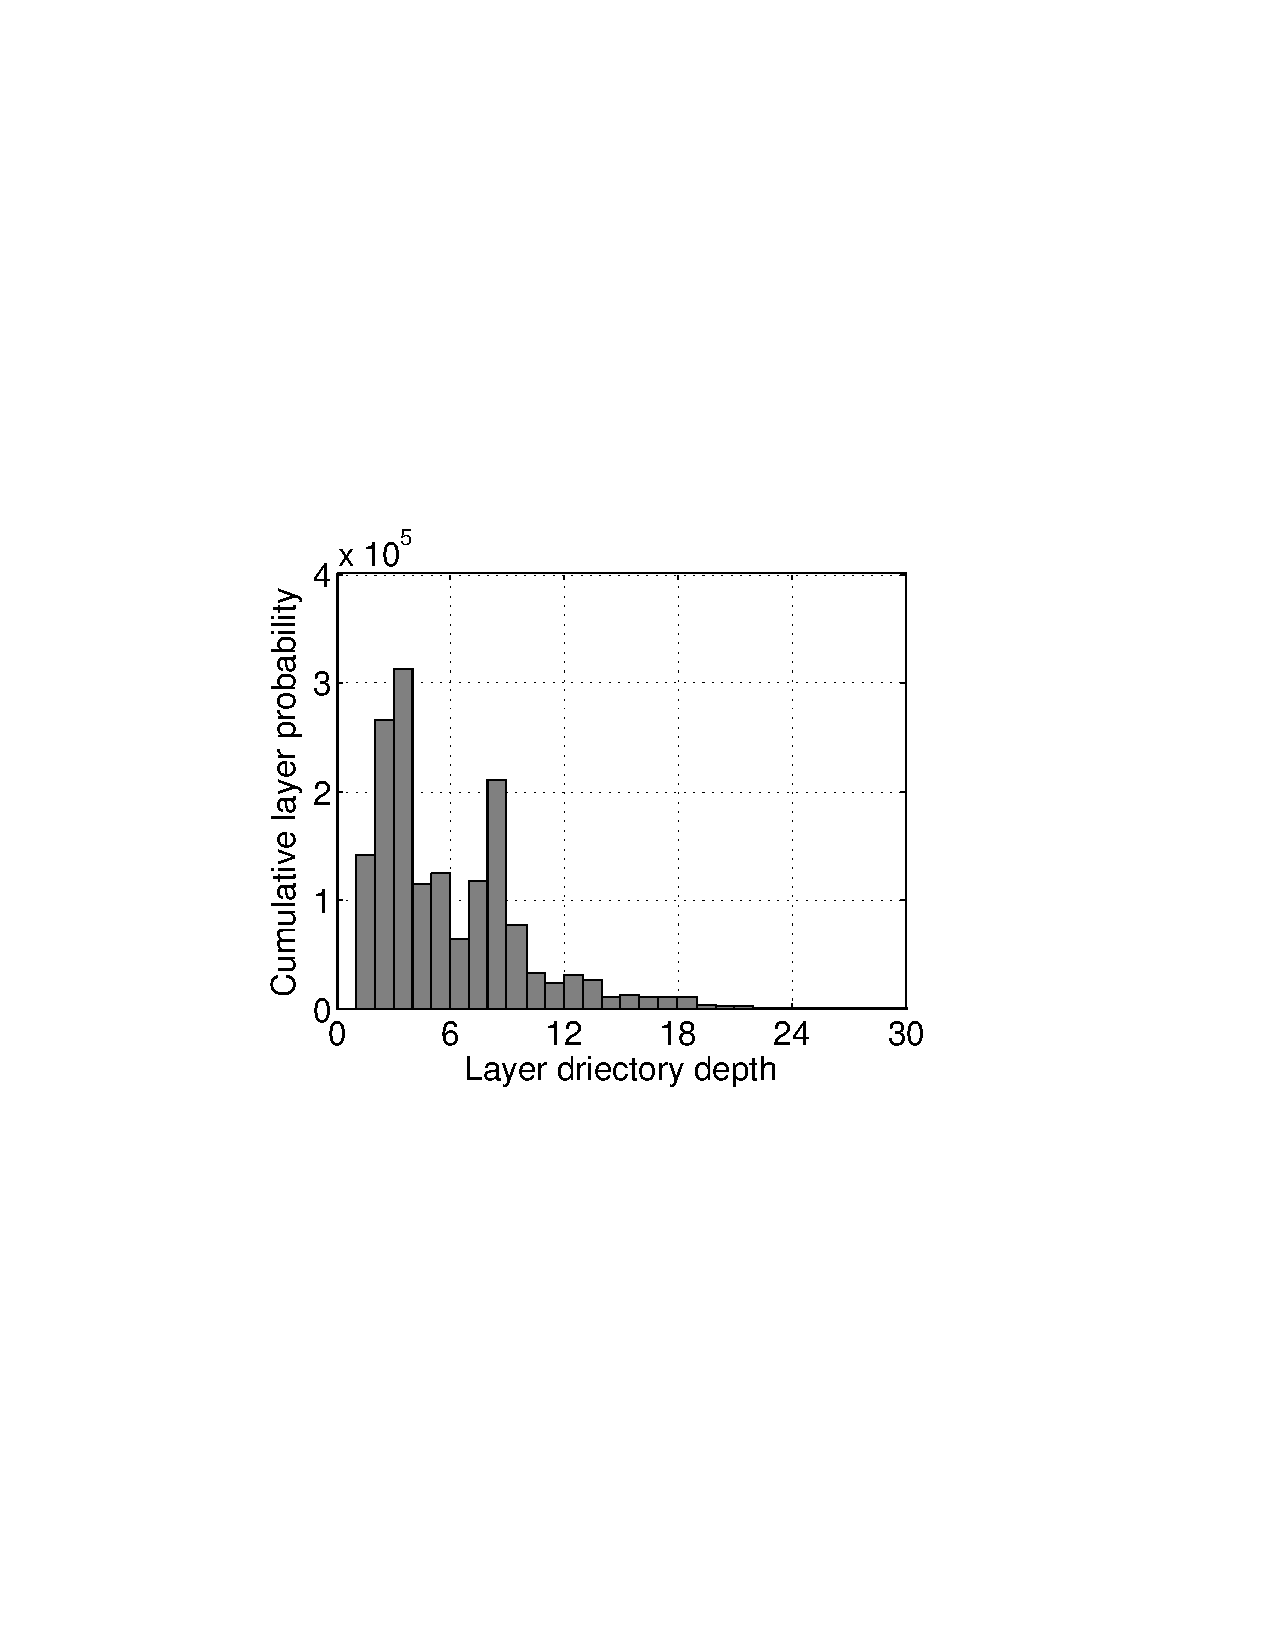
\includegraphics[width=0.22\textwidth]{graphs/hist_layer_depth.pdf}
	}
	\caption{Layer directory depth distribution}
	\label{fig-layer-dir}
\end{figure}

\subsubsection{Directory count distribution}

Figure~\ref{fig_dir_cnt} shows the cumulative layer probability by directories. 90\% of images have less than 826 directories. Half of images have less than 11 directories. The maximum is 111,940 while the minimum is 1. The average is 273. 

\begin{figure}
	\centering
	\begin{minipage}{0.25\textwidth}
		\centering
		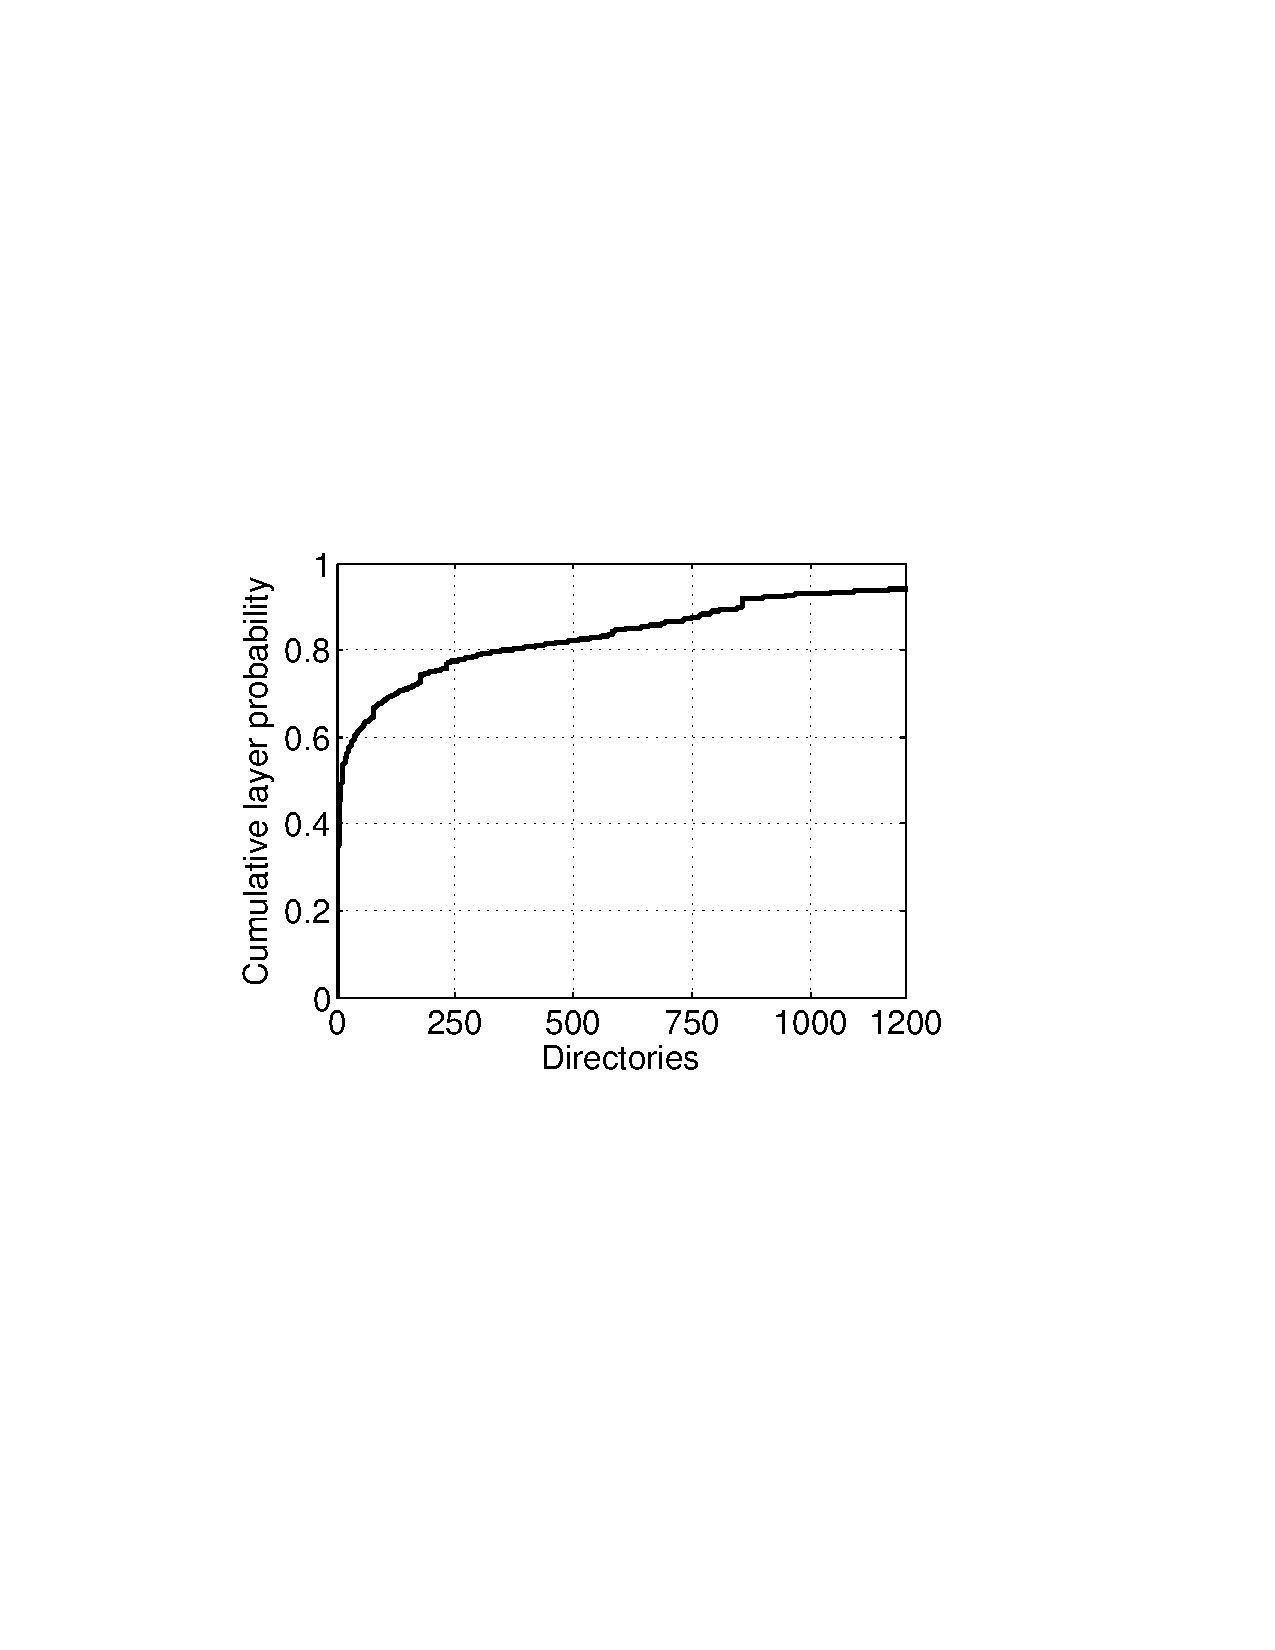
\includegraphics[width=1\textwidth]{graphs/dir_cnt.pdf}
		\caption{Directory count distribution}
		\label{fig_dir_cnt}
	\end{minipage}%
	\begin{minipage}{0.26\textwidth}
		\centering
		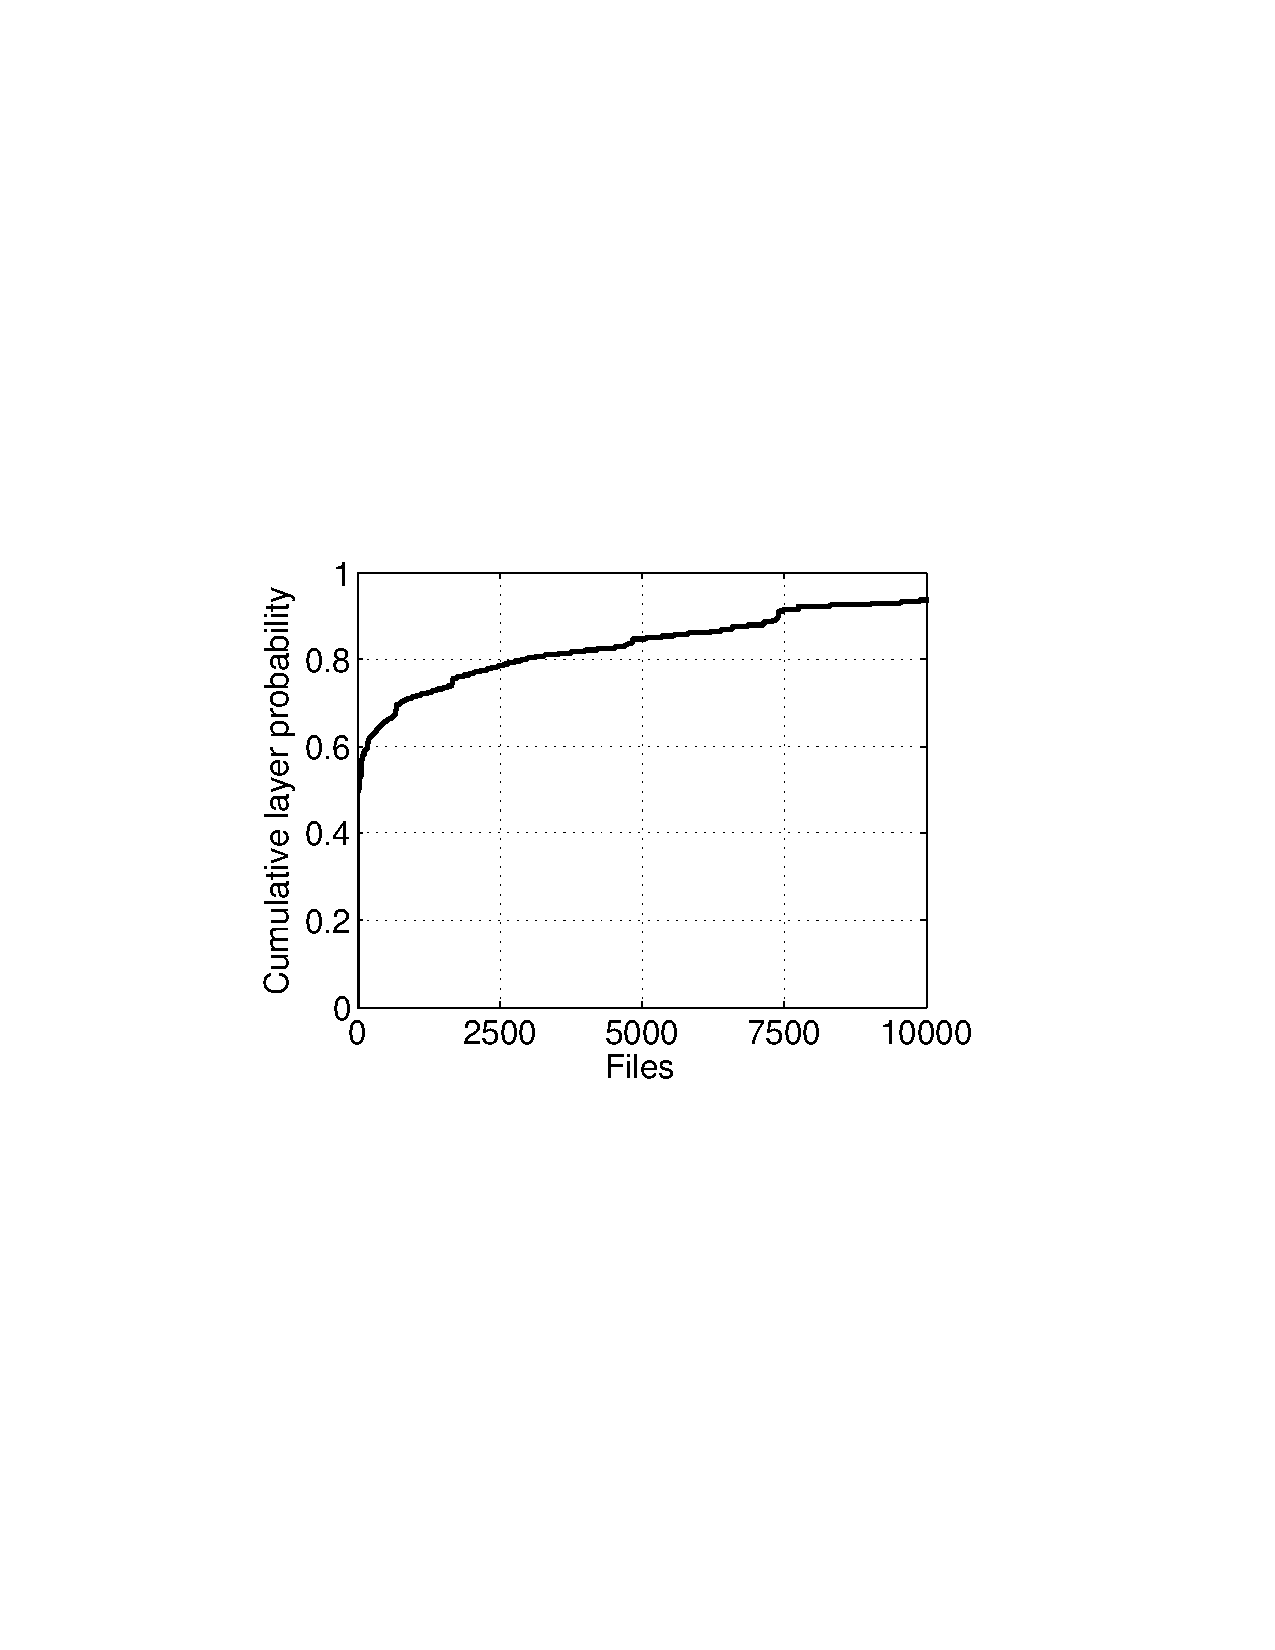
\includegraphics[width=1\textwidth]{graphs/file_cnt.pdf}
		\caption{File count distribution}
		\label{fig_file_cnt}
	\end{minipage}
\end{figure}

\subsubsection{File count distribution}

Figure~\ref{fig_file_cnt} shows the cumulative image frequency by files. 90\% of images have less than 7,410 files. Half of images have less than 30 files. The maximum is 826,196 while the minimum is 1. The average is 2,200.

\subsection{File}

\subsubsection{File size distribution}

\begin{figure}[!t]
	\centering
	\subfigure[CDF of files by file size (KB)]{\label{fig_cdf_file_size_kb}
		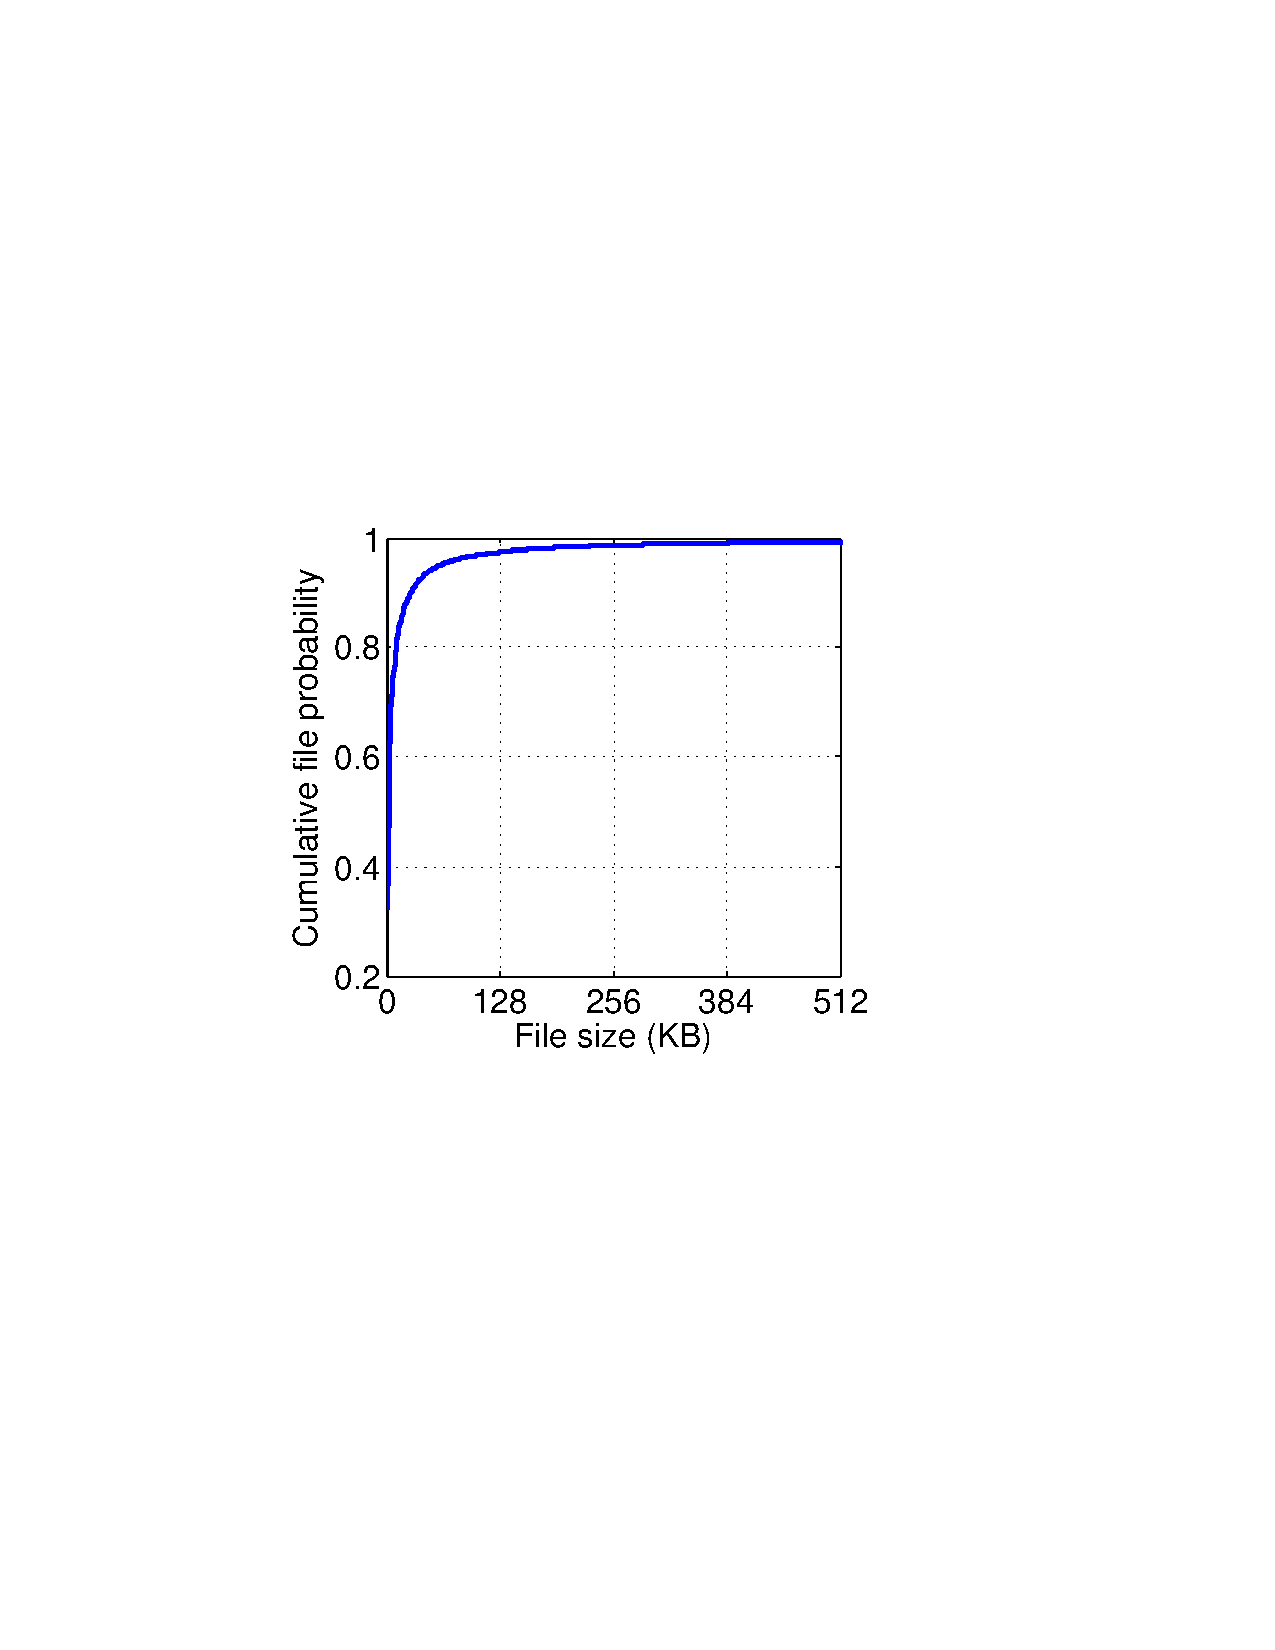
\includegraphics[width=0.23\textwidth]{graphs/cdf_file_size_kb.pdf}
	}
	\subfigure[Histogram of files by file size (KB)]{\label{fig_hist_file_size_kb}
		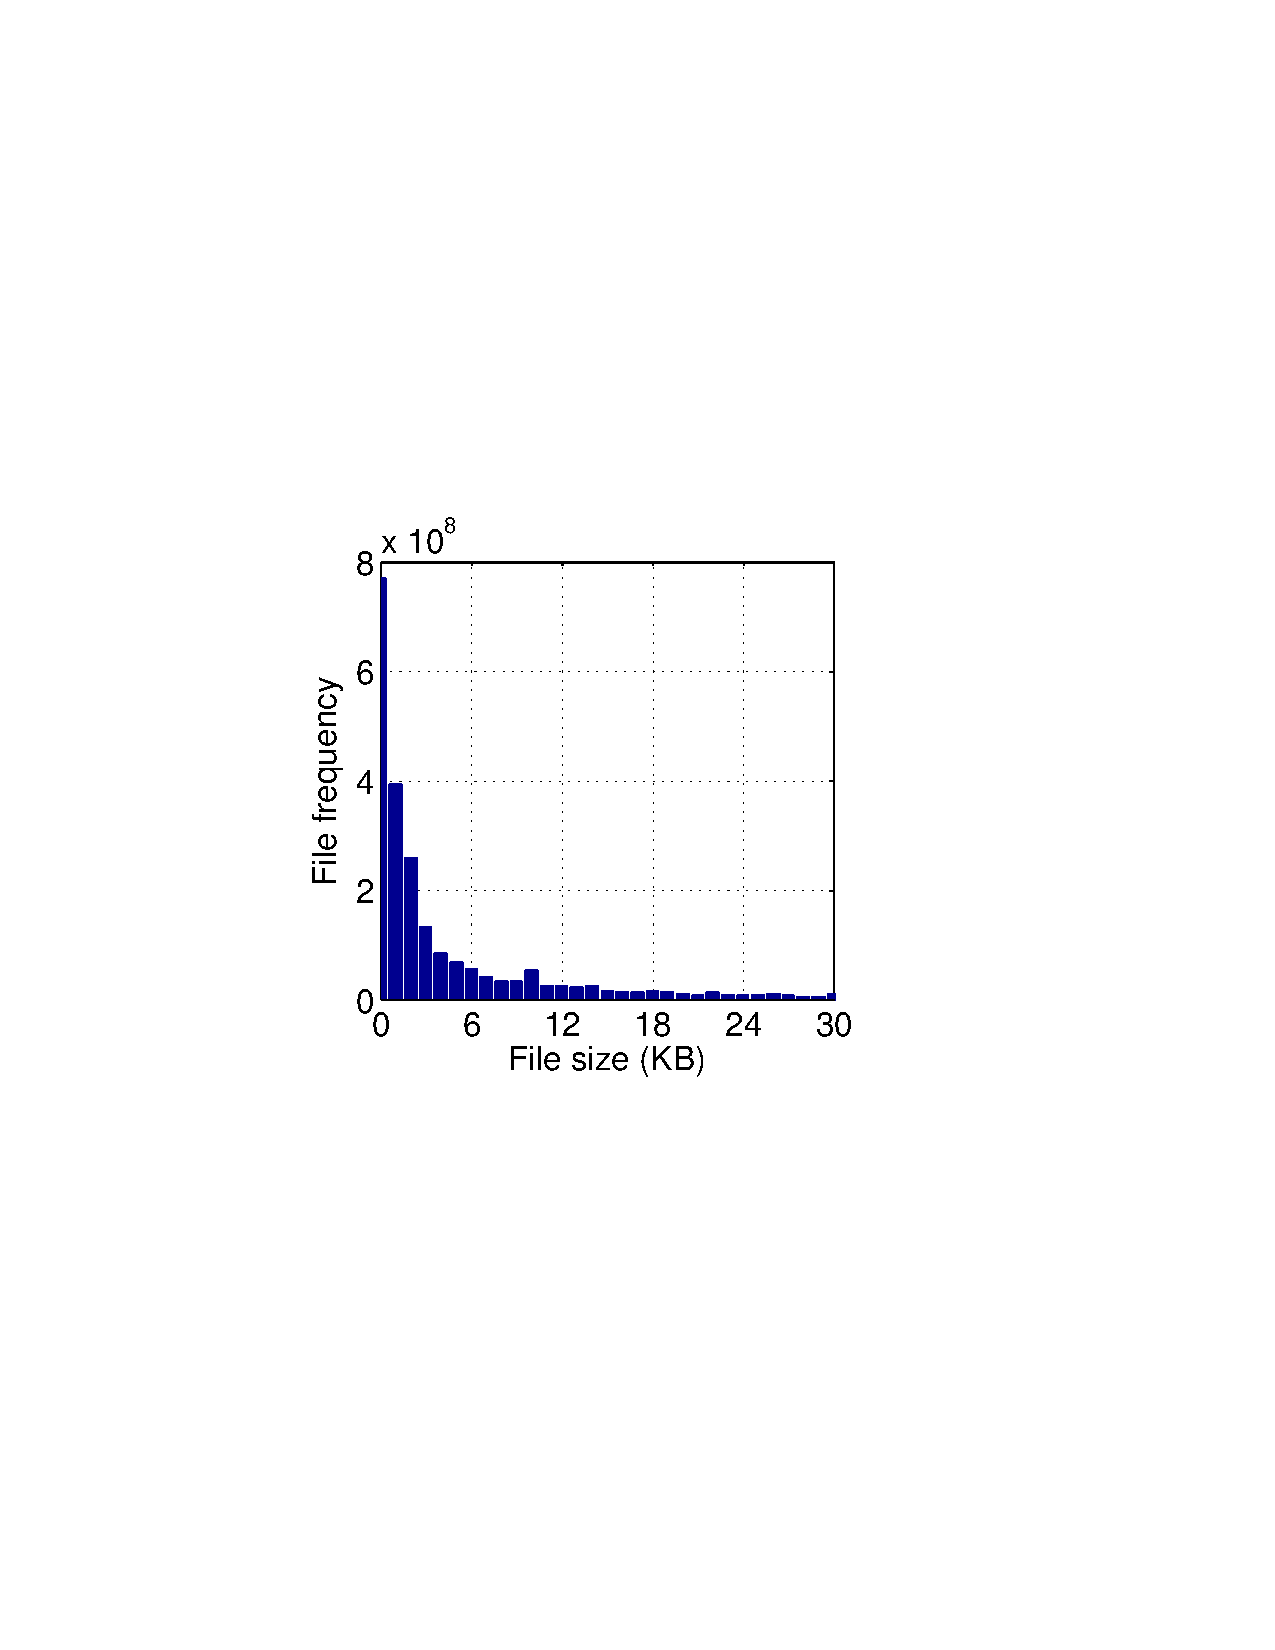
\includegraphics[width=0.22\textwidth]{graphs/hist_file_size_kb.pdf}
	}
	\caption{File size distribution}
	\label{fig-file-size}
\end{figure}

Figure~\ref{fig_cdf_file_size_kb} shows the cumulative file probability by file size. Around 90\% of layers' directory depth is less than 30 KB. 50\% of layers' directory depth is less than ~3. Figure~\ref{fig_hist_file_size_kb} shows the histogram of files by file size. About 769,000,000 files' size is less 1 KB, which is the peak value in the figure. The maximum file size is ~12GB.

Figure~\ref{fig-file-size} suggests that majority of files in Docker images are small files. About 30\% of files are less than 1 KB. 99\% of files are smaller than 1 MB.

\subsubsection{File type distribution}

We use python library named python-magic~\cite{python-magic} to obtain the file type. Overall, there are 3,006,619,271 regular files and 282,379,663 symbolic links. Figure~\ref{fig-file-type} shows the top 22 file types. As shown, ASCII text is the most popular file type in Docker images. Around 886,843,570 (30\%) of files are ASCII text files. 
About 322,404,420 (11\%) files are gzip compressed files 
Interestingly, about 22,492,597 (1\%) of files are empty.  

\begin{figure*}
	\centering
	% Requires \usepackage{graphicx}
	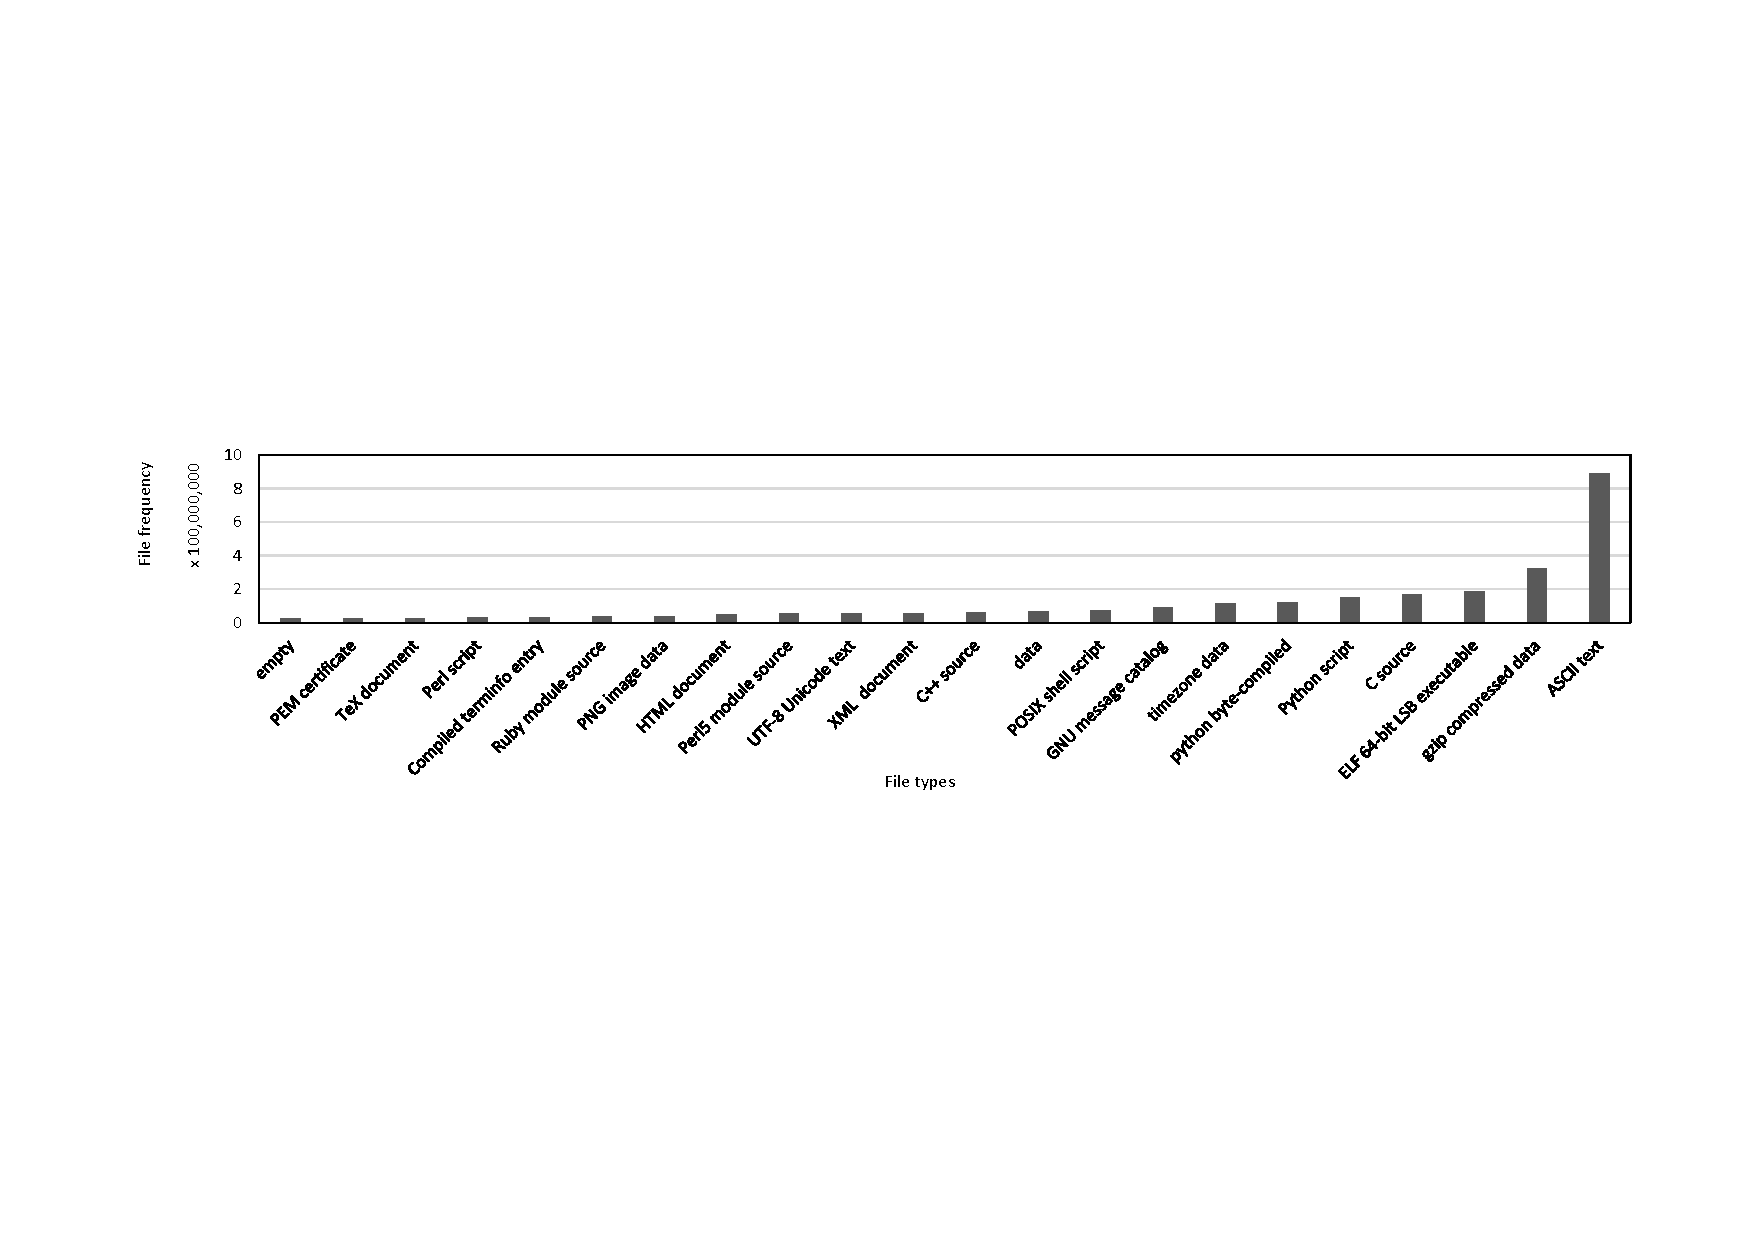
\includegraphics[width=1\textwidth]{graphs/file_type.pdf}\\
	\caption{File type distribution}\label{fig-file-type}
\end{figure*}
